\section{Experiment}
\label{sec:experiment}
% \subsection{Experiment setup}
\noindent{\textbf{Dataset}} We validate our ideas on NuScenes dataset~\cite{caesar2020nuscenes} where full 360-degree coverage provided by six cameras is available. Specifically, it consists of 1000 examples of street-view scenes in Boston and Singapore, each of which lasts for 20s and is captured at 12Hz. Besides 1.4M camera images, NuScenes also provides multi-modal data, including both global map layers and 3D object bounding boxes annotated on 40k keyframes. 
% NuScenes also provides multi-modal data, including LIDAR and RADAR sweeps, as well as map layers. More importantly, 3D object bounding boxes are annotated 40k keyframes. 
We follow the standard split of 700/150/150 for training, validation, and testing. We report our results on the validation set of Nuscenes and follow the split of~\cite{caesar2020nuscenes} where 600 sets of images are used. 

\begin{table*}[h!]
    \centering
    \caption{Quantitative results and human analysis on NuScenes. We observe a noticeable superiority of our MVPbev. %over existing methods.
    % Numbers show the winning percent of left column methods vs top row methods 
    }
    \resizebox{\textwidth}{!}{
    
% \subfloat[Quantitative results on NuScenes dataset]{
% \begin{tabular}{c|ccc|c|c} 
% \hline
% \multirow{2}{*}{Method} & \multicolumn{3}{c|}{Image Quality} & Semantics Consistency & Visual Consistency \\ 
% \cline{2-6}
%  & FID$\downarrow$ & IS$\uparrow$ & CS$\uparrow$ & $\rm{IoU_{BEV}}$$\uparrow$ & PSNR$\uparrow$ \\ 
% \hline
% Reference-score & $18.87$ & $ 4.53 $ & $25.94$ & $0.711$ & $15.37$ \\ 
% Controlnet~\cite{zhang2023adding} & $21.93$ & $4.71$ & $27.02$ & $0.434$ & $12.82$ \\ 
% MVD~\cite{Tang2023mvdiffusion} & $19.89$ & $4.91$ & $27.07$ & $0.440$ & $12.66$ \\
% BEVGen\cite{swerdlow2023street} & $25.54$ & - & - & $0.502$ & - \\
% MagicDrive\cite{gao2023magicdrive} & $\mathbf{16.20} $ & - & - & $\mathbf{0.611}$ & - \\
% \hline
% Ours & $16.95$ & $\mathbf{6.35}$ & $\mathbf{28.79}$ & 0.510 & $\mathbf{20.67}$ \\
% \hline
% \end{tabular}
% }

\subfloat[Quantitative results on NuScenes dataset]{
\begin{tabular}{c|c|ccc|c|c} 
\hline
\multirow{2}{*}{Method} & \multirow{2}{*}{Training Samples} & \multicolumn{3}{c|}{Image Quality} & Semantics Consistency & Visual Consistency \\ 
\cline{3-7}
 & & FID$\downarrow$ & IS$\uparrow$ & CS$\uparrow$ & $\rm{IoU_{BEV}}$$\uparrow$ & PSNR$\uparrow$ \\ 
\hline
Reference-score & - &$6.20$ & $ 5.77 $ & $27.54$ & $0.711$ & $15.37$ \\ \hline \hline
BEVGen\cite{swerdlow2023street} & $28130$ & $25.54$ & - & - & $0.502$ & - \\
MagicDrive\cite{gao2023magicdrive} & $28130$ & $\mathbf{16.20} $ & - & - & $\mathbf{0.611}$ & - \\ \hline
Controlnet~\cite{zhang2023adding} & $6000$ & $21.93$ & $4.71$ & $27.02$ & $0.434$ & $12.82$ \\ 
MVD~\cite{Tang2023mvdiffusion} & $6000$ & $19.89$ & $4.91$ & $27.07$ & $0.440$ & $12.66$ \\
\hline \hline
Ours & $6000$ & $16.95$ & $\mathbf{6.35}$ & $\mathbf{28.79}$ & 0.510 & $\mathbf{20.67}$ \\
\hline
\end{tabular}
}


\quad

\subfloat[Human analysis on NuScenes dataset. ]{
\begin{tabular}{cc|ccc}
\hline
\multicolumn{2}{c|}{Comparisons}                                                                                              & Win & Undecided & Lose \\ \hline \hline
\multicolumn{1}{c|}{\multirow{3}{*}{\begin{tabular}[c]{@{}c@{}}Cross-view\\ Consistency\end{tabular}}} & MVD v.s. Controlnet  & $\mathbf{.26}$ & $.50$       & $.25$  \\
\multicolumn{1}{c|}{}                                                                                  & Ours v.s. Controlnet & $\mathbf{.73}$ & $.27$       & $.00$  \\
\multicolumn{1}{c|}{}                                                                                  & Ours v.s. MVD        & $\mathbf{.71}$ & $.29$       & $.00$  \\ \hline \hline
\multicolumn{1}{c|}{\begin{tabular}[c]{@{}c@{}}Camera Pose\\ Consistency\end{tabular}}                 & Ours v.s. MagicDrive & $\mathbf{.61}$ & $.31$       & $.08$    \\ \hline
\end{tabular}
}

% \subfloat[Human analysis on NuScenes dataset. ]{
% \begin{tabular}{c|c|ccc}
%     \toprule
%     \multicolumn{2}{c|}{Comparisons} & Win & Undecided & Loss \\
%     \midrule
%     \multirow{3}{}{Cross-view consistency}
%     MVD~\cite{Tang2023mvdiffusion} v.s. Controlnet~\cite{zhang2023adding} & .26 & .50 & .25 \\
%     Ours v.s. Controlnet~\cite{zhang2023adding} & .73 & .27 & .00 \\
%     Ours v.s. MVD~\cite{Tang2023mvdiffusion} & .71 & .29 & .00 \\
%     \hline 
    
% \end{tabular}
% }


% original table 1
% \begin{table*}%[H]
%            \centering
%            \captionsetup[subtable]{position = below}
%           \captionsetup[table]{position=top}
%            \caption{Blahblah}
%            \begin{subtable}{0.3\linewidth}
%                \centering
%                \begin{tabular}{|c|c|}
%                    \hline
%                    \textbf{h [m]} & \textbf{dim [m]} \\ \hline
%                    30 & 0.75 \\ \hline
%                    50 & 1.25 \\ \hline
%                    70 & 1.75 \\ \hline
%                    100 & 2.50 \\ \hline
%                \end{tabular}
%                \caption{Minimum dimension of an object for it to be detected by the FFT algorithm at different heights}
%                \label{tab:dimFFT}
%            \end{subtable}%
%            \hspace*{4em}
%            \begin{subtable}{0.3\linewidth}
%                \centering
%                \begin{tabular}{|c|c|}
%                    \hline
%                    \textbf{h [m]} & \textbf{dim [m]} \\ \hline
%                    30 & 0.28 \\ \hline
%                    50 & 0.47 \\ \hline
%                    70 & 0.66 \\ \hline
%                    100 & 0.94 \\ \hline
%                \end{tabular}
%                 \caption{Minimum dimension of an object for it to be detected by the GMM algorithm at different heights}
%                  \label{tab:dimGMM}
%            \end{subtable}
%        \end{table*}


% %% side by side using parbox
% \parbox{.45\linewidth}{
% \centering

% \begin{tabular}{c|ccc|cc|c} 
% \hline
% \multirow{2}{*}{Method} & \multicolumn{3}{c|}{Image Quality} & \multicolumn{2}{c|}{Semantics Consistency} & Visual Consistency \\ 
% \cline{2-7}
%  & FID$\downarrow$ & IS$\uparrow$ & CS$\uparrow$ & $\rm{IoU_{Pers}}$$\uparrow$ & $\rm{IoU_{BEV}}$$\uparrow$ & PSNR$\uparrow$ \\ 
% \hline
% Reference-score & $18.87$ & $ 5.11 $ & $26.46$ & $0.618$ & $0.711$ & $15.37^*$ \\ 
% SD + Controlnet~\cite{??} & $\mathbf{32.71}$ & $\mathbf{3.53}$ & $28.66$ & $0.476$ & $0.366$ & $12.08$ \\ 
% MVDiffusion~\cite{??} & $43.83$ & $3.11$ & $28.69$ & $0.560$ & $0.418$ & $11.64$ \\ 
% \hline
% Ours & $38.22$ & $3.25$ & $\mathbf{28.71}$ & $\mathbf{0.588}$ & $\mathbf{0.421}$ & $\mathbf{20.05}$ \\
% \hline
% \end{tabular}

% \caption{1. xxxxxxxxxxxxxxxxxxxxxx}
% }

% \hfill


% \parbox{.45\linewidth}{
% \centering

% \begin{tabular}{c|ccc}
%     \toprule
%      Comparisons & Win & Undecided & Loss \\
%     \midrule
%     MVDiffusion~\cite{??} v.s. SD + Controlnet~\cite{??} & .26 & .50 & .25 \\
%     Ours v.s. SD + Controlnet~\cite{??} & .73 & .27 & .00 \\
%     Ours v.s. MVDiffusion~\cite{??} & .71 & .29 & .00 \\
%     \hline 
    
% \end{tabular}

% \caption{2. xxxxxxxxxxxxxxxxxxx}
% }
    }
    \label{tbl:qualitative}
\end{table*}

\begin{figure*}[t]
\centering
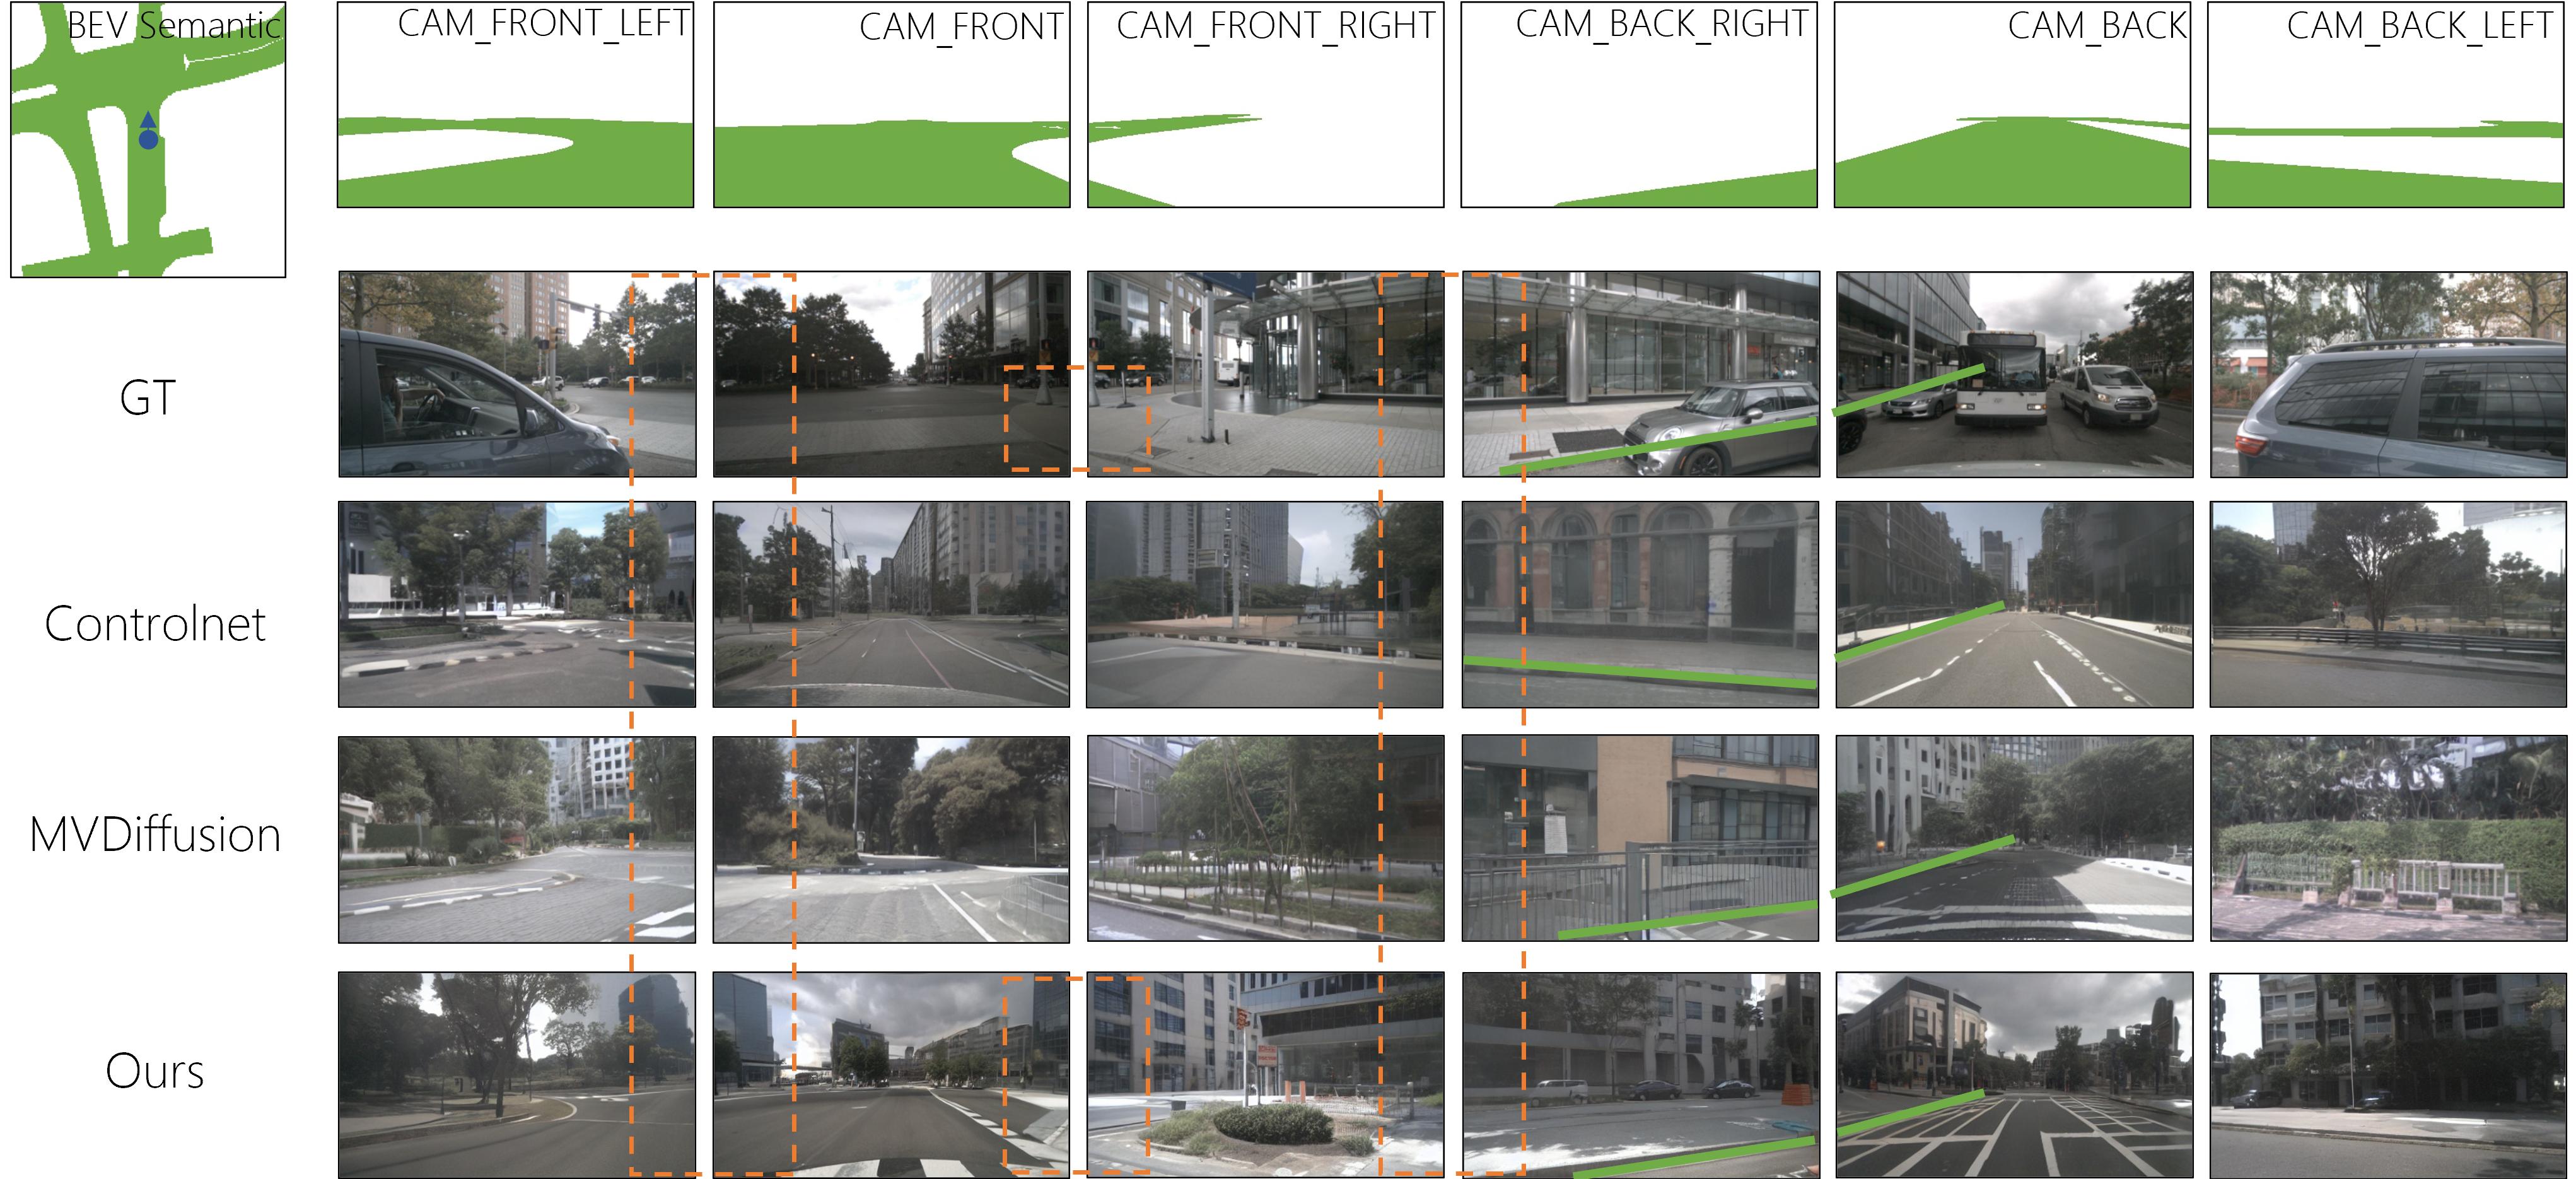
\includegraphics[width=0.95\linewidth]{figures/qualitative_comparison.png}
\caption{Our MVPbev is able to achieve the most visual and semantic consistent images w.r.t. input control signal. We highlight the overlapping area and road boundary in orange bounding boxes and green lines. 
}
\label{fig:quali_comp}
\end{figure*}

\noindent{\textbf{Evaluation metrics}} We follow~\cite{Tang2023mvdiffusion} to include the image quality of generated images and their visual consistency in our evaluation metrics. In addition, semantic consistency is also valued to reflect the synthesis quality of different semantic categories.

\begin{packed_lefty_item}
\item \textit{Image quality} is measured by Fréchet Inception Distance (FID)~\cite{cortes2015advances}, Inception Score (IS)~\cite{salimans2016improved}, and CLIP Score (CS)~\cite{radford2021learning}. In particular, FID is based on the distribution similarity between the features of the generated and real images. The IS measures the diversity and predictability of generated images. Finally, CS measures the text-image similarity according to pre-trained CLIP models~\cite{radford2021learning}.

\item \textit{Visual consistency} provides pixel-wise similarity measurements on overlapping regions. We borrow the idea from Peak Signal-to-Noise Ratio (PSNR) where we first compute this PSNR between all the overlapping regions, and then compare this “overlapping PSNR” for ground truth images and generated images. The higher this value is, the better visual consistency will be. Note that the process of computing "overlapping PSNR" is based on estimated homography matrices, it's possible that generated image yields higher values than the ground truth image.

\item \textit{Semantic consistency} measures the pixel-wise semantic consistency between generated images and ground truth. In our case, we utilize the Intersection-over-Union (IoU) score. Particularly, we report the semantic IoU both in perspective view and BEV. As for the former, we apply pre-trained segmentation model~\cite{cheng2022masked} on generated images, leading to semantic predictions in perspective view. These predictions are then compared with $\{S_m\}_m$ to obtain IoU in perspective view. As for the latter, we apply pre-trained CVT~\cite{zhou2022cross} to generated images and the BEV IoU is obtained by comparing predictions from CVT with $\textit{B}$.

\item \textit{Object-level controllability} measures how accurately the object-instance is generated w.r.t. test-time descriptions. Here we report the averaged color distance Delta-E in CIELAB color space as well as their standard deviations.  
\end{packed_lefty_item}

Besides these metrics, we also perform human analysis. We request humans to decide which method is more visually realistic and consistent when results from different methods are provided. %Please note that 
Methods are anonymous to humans and when compared. And we ensure that the same input control signals are provided to various methods. Meanwhile, we also conduct experiments with instance-level controllability. Humans are provided with objects as well as their targeted color, paired with the generated images. And they will vote on whether the generated objects meet the requirements.
% Specifically, given the same input control signal, we can obtain multi-view images from all methods. Humans are fed with two sets of generated images from two different methods and then asked to make pairwise comparisons about which set is better, based on their visual qualities. 

\begin{figure*}[t]
\centering
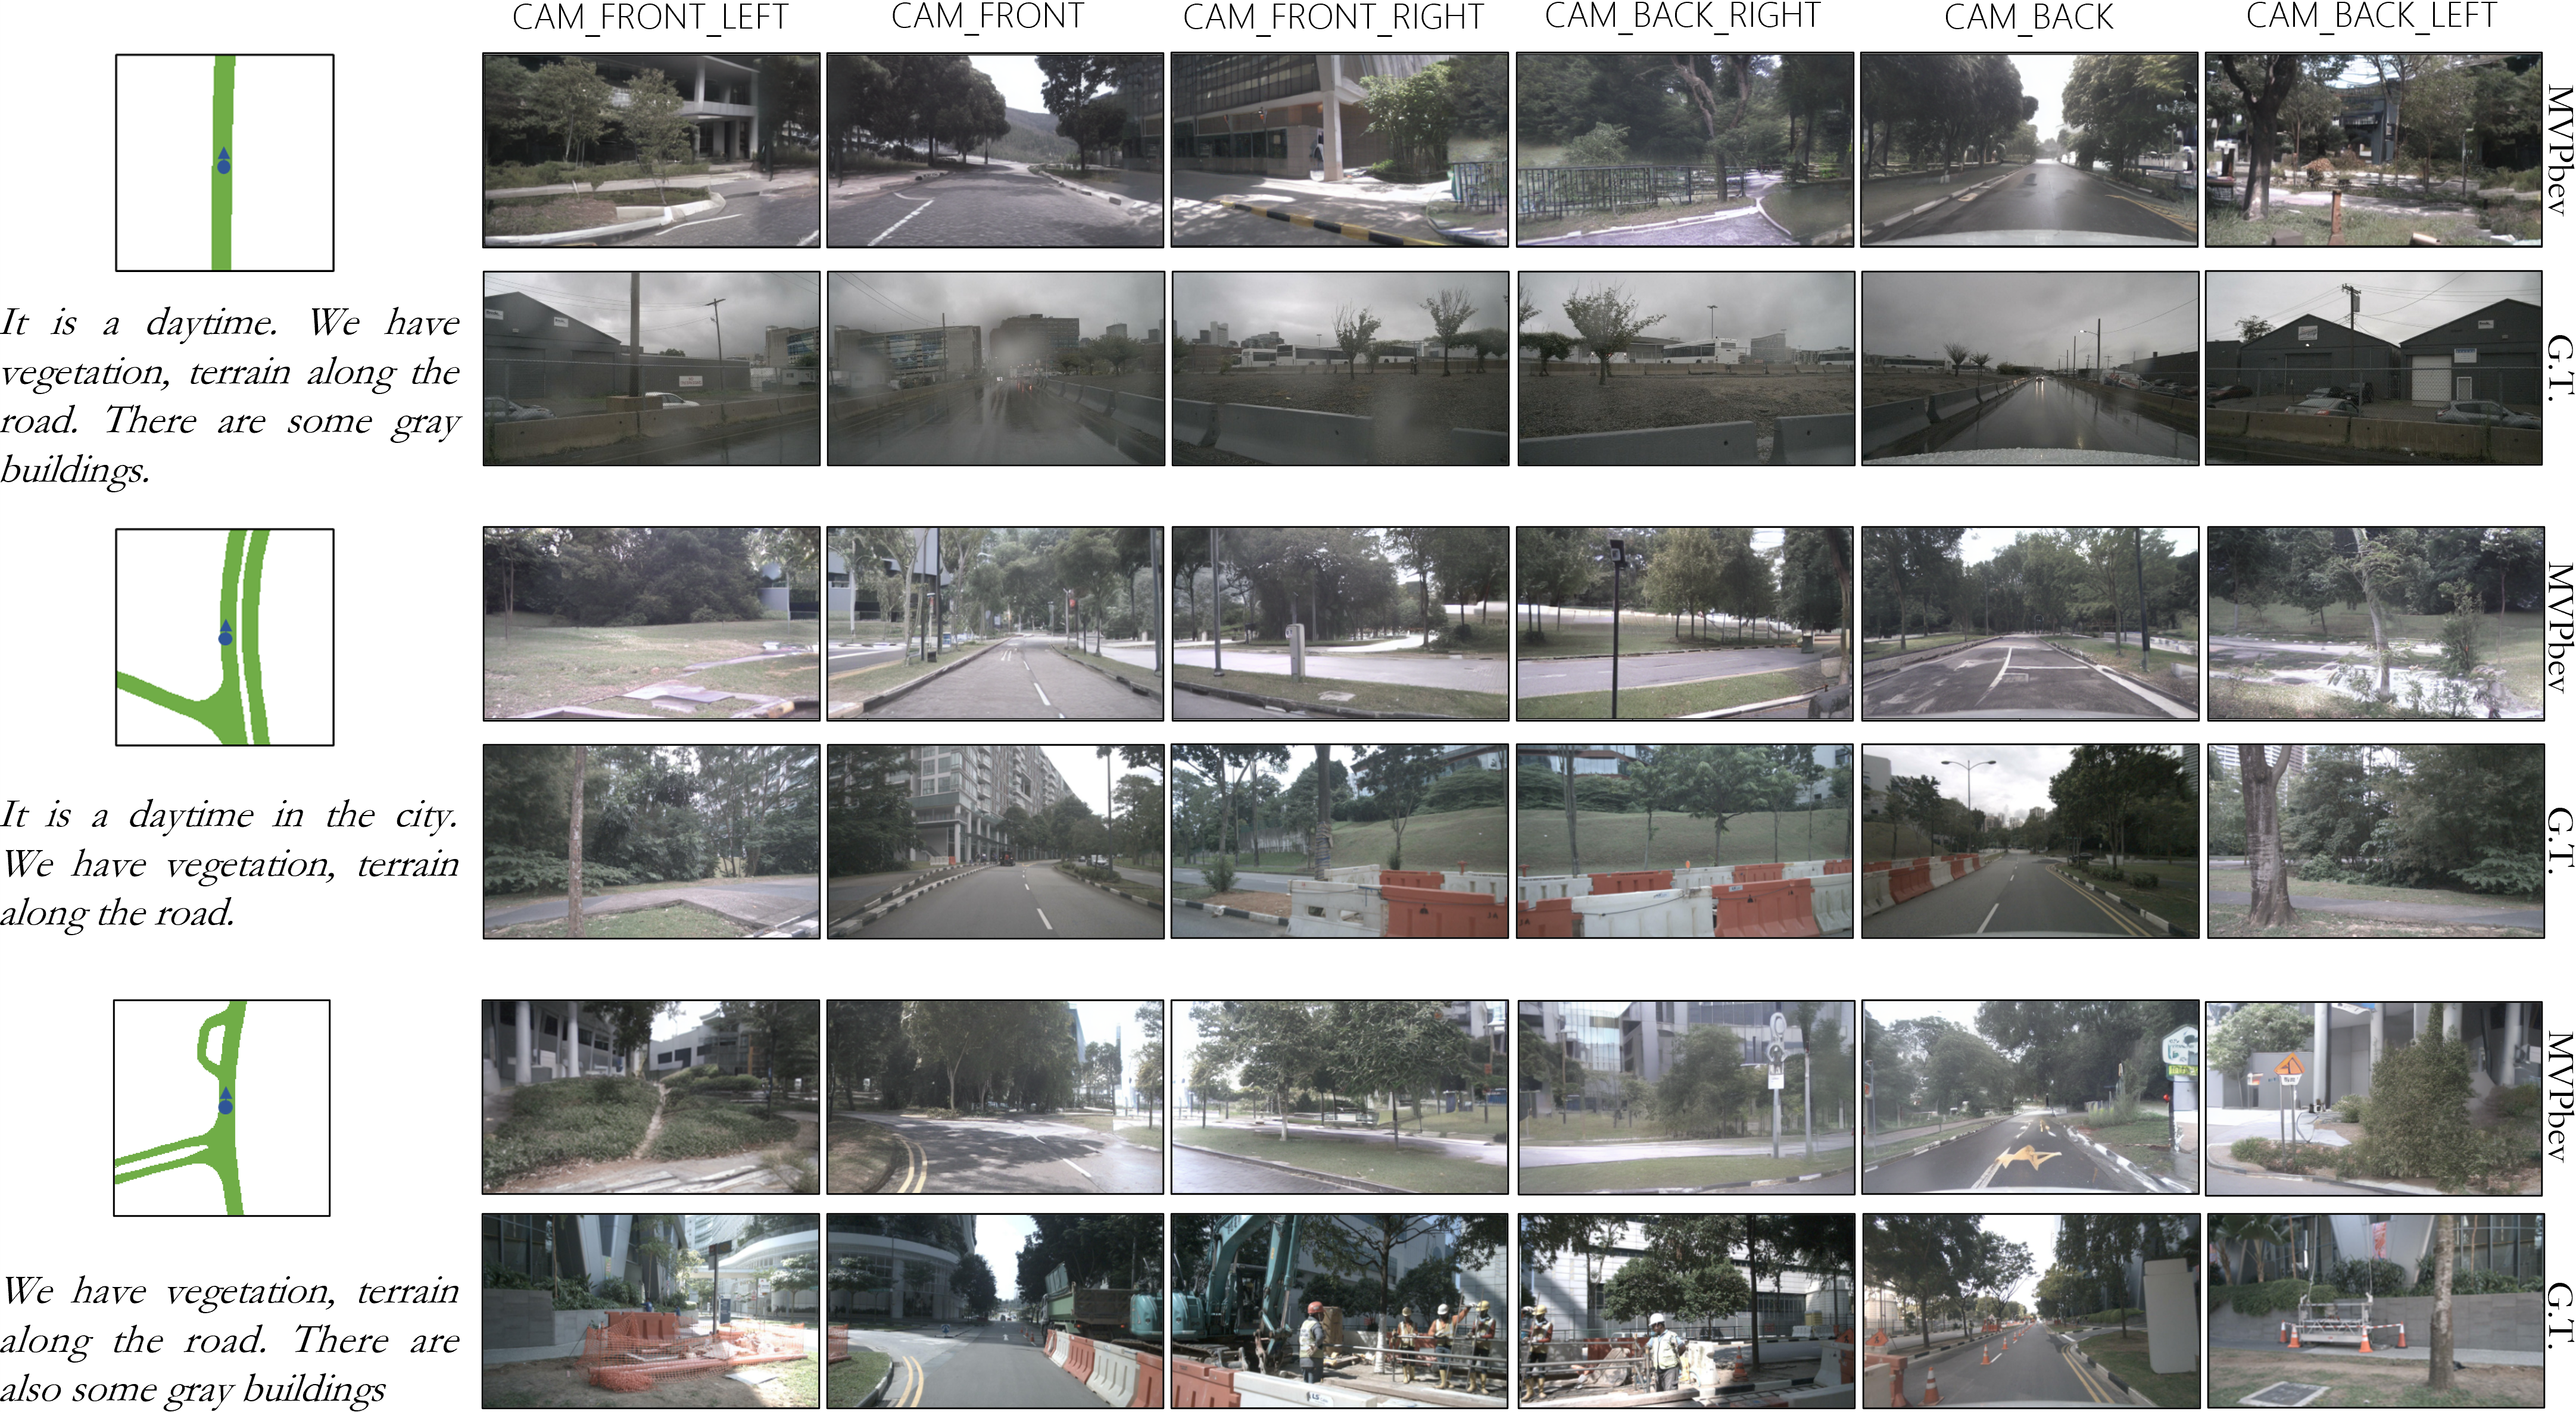
\includegraphics[width=0.95\linewidth]{figures/demo.png}
\caption{Qualitative results of MVPbev. We provide three sets of examples. The leftmost column consists of input signals, while the 2nd to 7th columns are images from different perspective views.
}
\label{fig:demo}
\end{figure*}

\noindent{\textbf{Baselines}} We select the following four state-of-the-art methods as our baselines for thorough comparisons:
\begin{packed_lefty_item}
\item \textit{SD+ControlNet}~\cite{rombach2021highresolution, zhang2023adding} is a basic yet powerful image generation model. Specifically, we work on the projected $\{S_m\}_m$ to avoid domain gaps from different viewpoints. Starting from a pre-trained ControlNet~\cite{zhang2023adding}, this baseline is fine-tuned on NuScenes training.  
\item \textit{MVDiffusion}~\cite{Tang2023mvdiffusion} is proposed to generate multi-view consistent images. % and achieves good performance on tasks like panoramic image generation. 
However, it is designed neither for dramatic view changes, e.g., BEV to perspective view, nor for semantic control signals. To this end, we %follow our pipeline to 
first map BEV semantics to perspective view and then update MVDiffusion with a pre-trained ControlNet~\cite{zhang2023adding} backbone. Specifically, We re-implement~\cite{Tang2023mvdiffusion} based on its official code and fine-tune it on NuScenes training images.
\item \textit{BEVGen}~\cite{swerdlow2023street} is the first step towards road scene generation, where the control signals are limited to BEV semantics and camera parameters. The full dataset is used for training. % And $28130$ set of images are used for training purposes.   
\item \textit{MagicDrive}~\cite{gao2023magicdrive}is the most recent published work on road scene generation. We use their released model for efficient comparison. Please note that we use only $20\%$ images uniformly sampled from dataset for training while they use the full dataset. % in their official implementation.
\end{packed_lefty_item}
% These four methods are chosen for performance and re-productivity purposes. We refer the readers to supplementary for full implementation details.

\subsection{Implementation Details}
Our BEV semantics $\textit{B}$ reflects an 80m $\times$ 80m space with ego car located at the center position. $c_b$ represents the drivable area in NuScenes. The resolution of the perspective image is $H\times W = 256\times 448$, leading to $h\times w = 32\times56$. As for the hyper-parameters, we set $M$ and $K$ to 6 and 3 respectively. We have implemented the system with PyTorch~\cite{paszke2019pytorch} while using publicly available Stable Diffusion codes~\cite{von-platen-etal-2022-diffusers}. Specifically, it consists of a denoising UNet to execute the denoising process within a compressed latent space and a VAE to connect the image and latent spaces. The pre-trained VAE of the Stable Diffusion is maintained with official weights and is used to encode images during the training phase and decode the latent codes into images during the inference phase. In experiments, we use a machine with 1 NVIDIA A40 GPU for training and inference. Batch size is set to 6 and $T$ equals to 50. We refer the readers to supplementary for full implementation details.

% \begin{figure*}[h]
% \centering
% 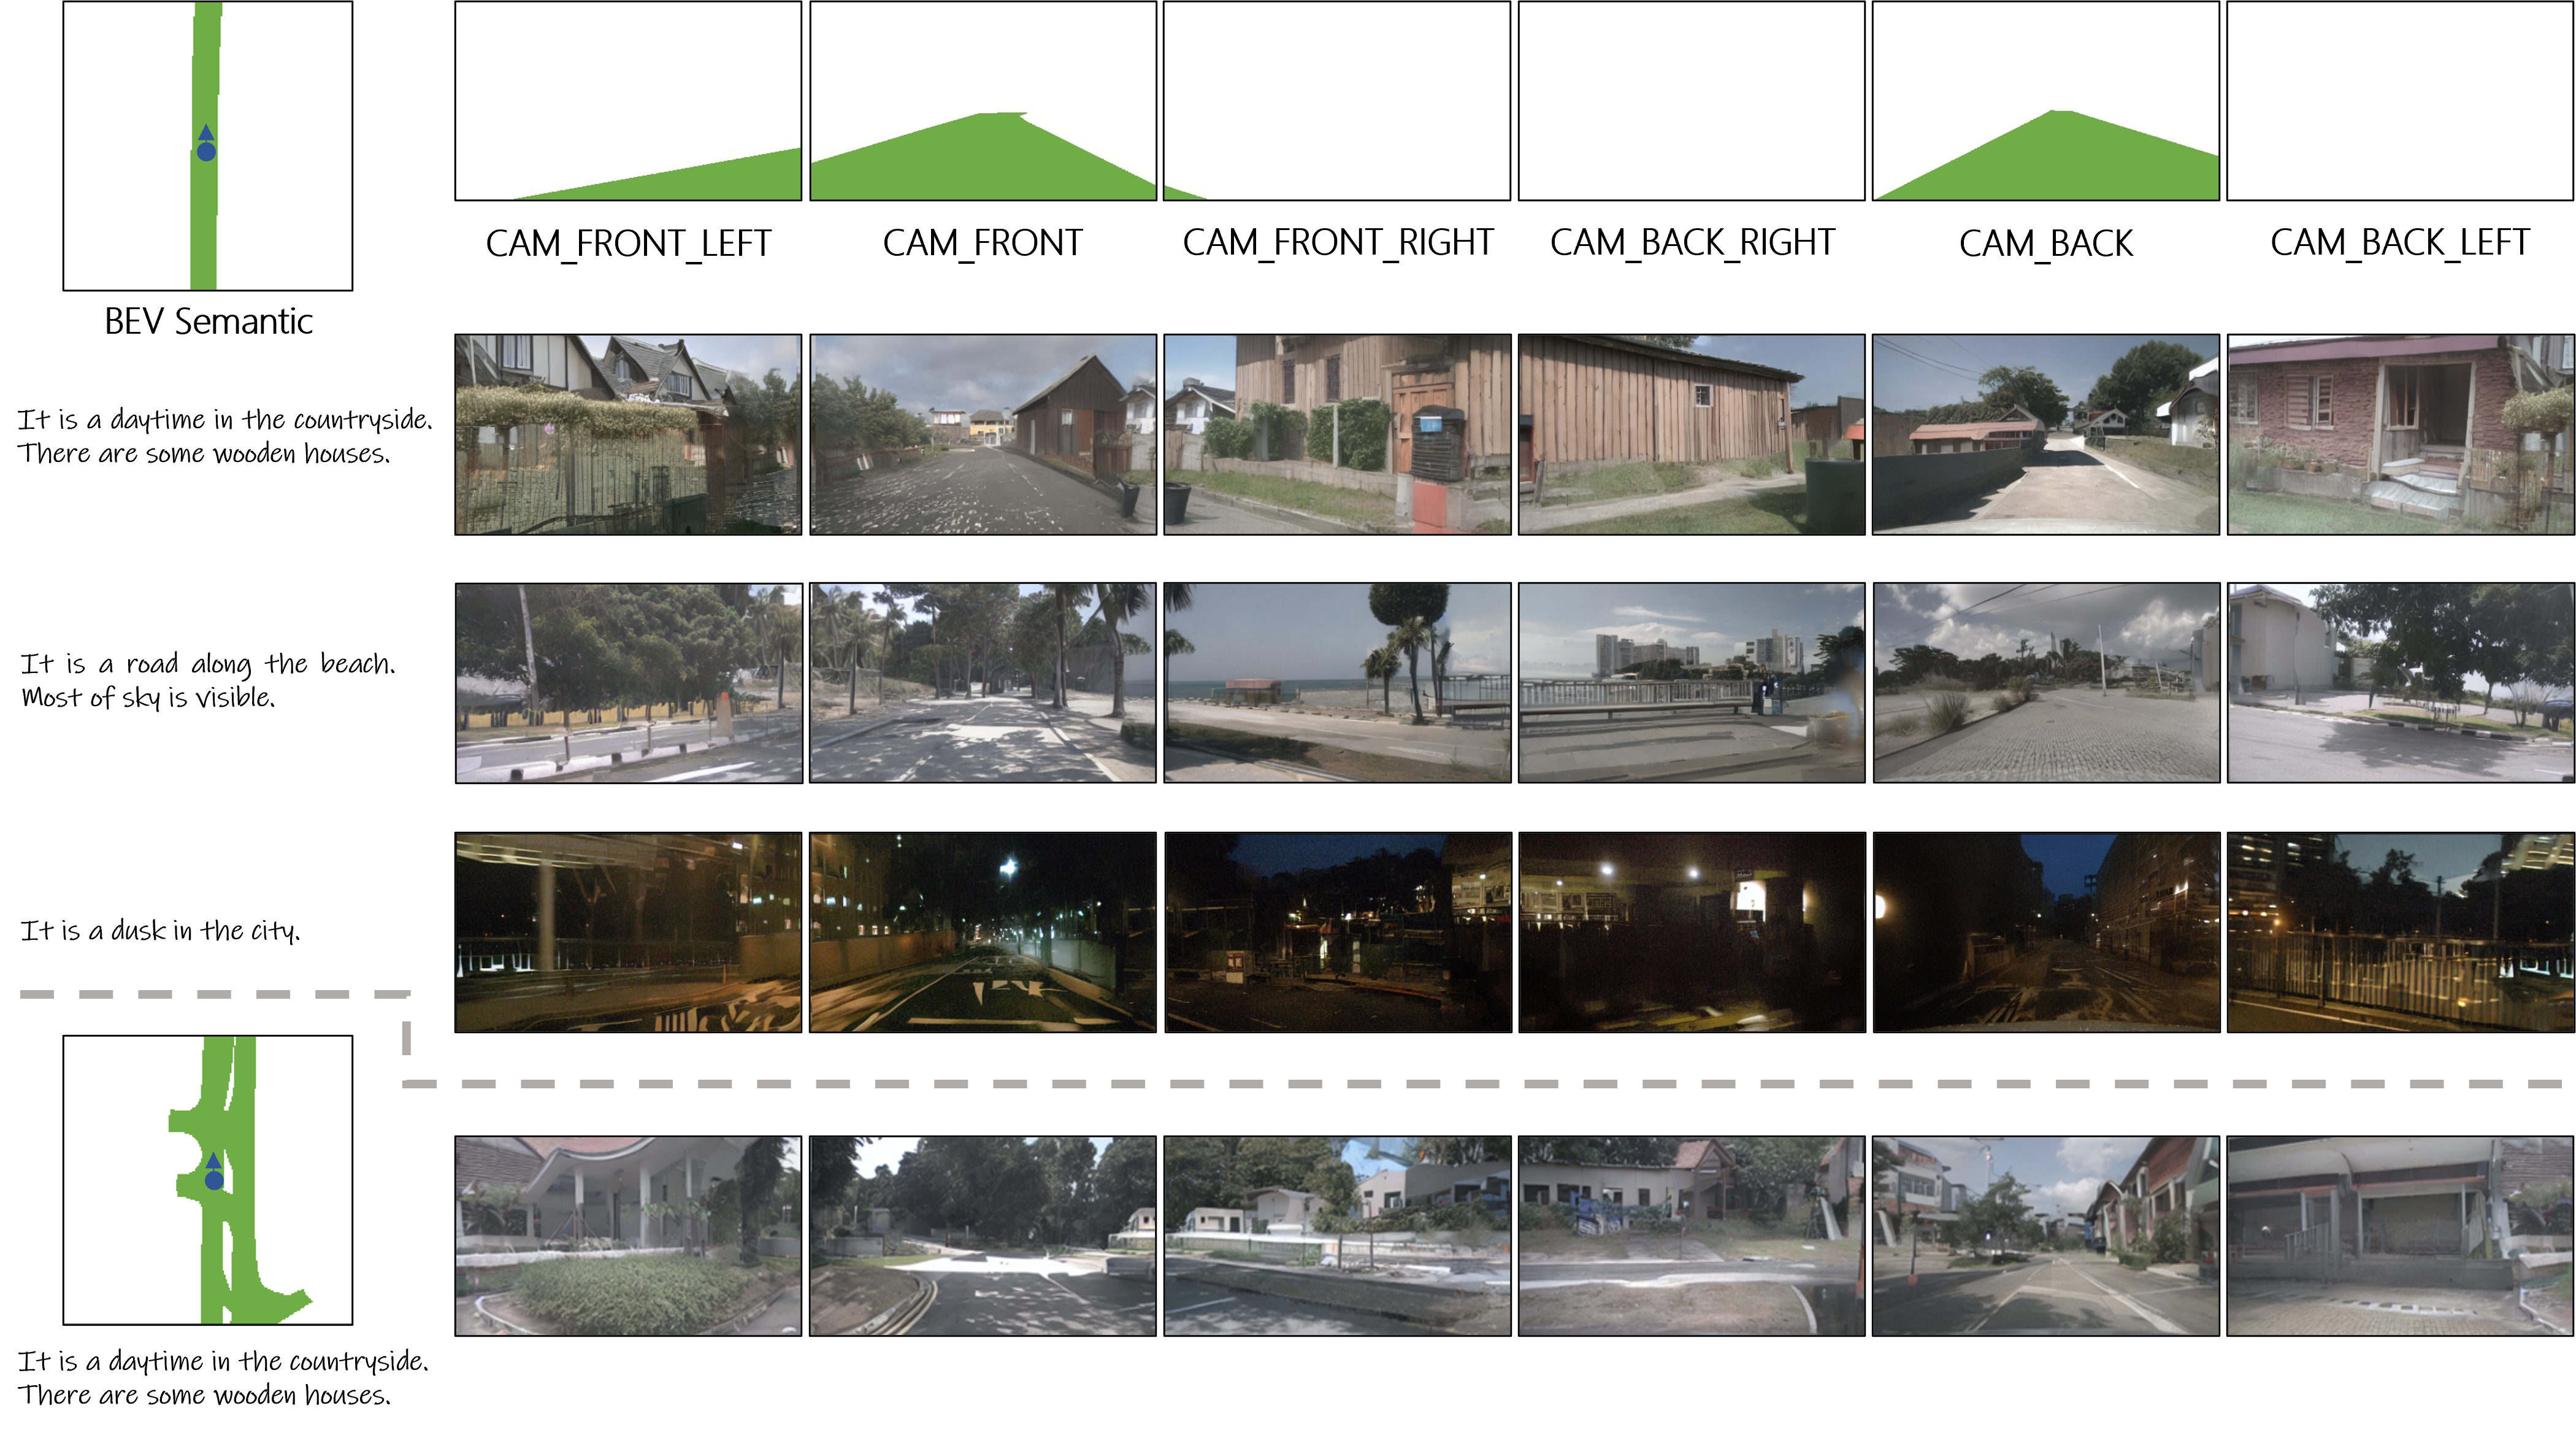
\includegraphics[width=\linewidth]{figures/fixed_bev_prompt_control.png}
% \caption{We are able to generate photo-realistic, diverse yet consistent multi-view perspective images with various control signals.
% }
% \label{fig:controllability}
% \end{figure*}

\begin{figure*}[t]
\centering
\includegraphics[width=0.95\linewidth]{figures/camera_pose_demo_semantic_overlay.jpg}
\caption{MVPbev is robust to camera pose changes without re-train the entire model, providing better test-time generalizability.
}
\label{fig:view_point}
\end{figure*}

\begin{figure}[h]
\centering
\includegraphics[width=0.9\linewidth]{figures/color_boxfig.png}
\caption{The Delta-E distance between the ground truth and generated color on our controlled instances.
}
\label{fig:obj_instance_eval}
\vspace{-2mm}
\end{figure}

\begin{figure}[b]
\centering
\includegraphics[width=0.9 \linewidth]{figures/mulit_obj_color_control_demo.png}
\caption{MVPbev is able to handle test-time instance-level controllability with various color requests.
}
\label{fig:obj_instance}
\end{figure}
\subsection{Multi-view BEV generation}
We compare our MVPbev with baselines and report the performance in Table~\ref{tbl:qualitative}. The first row in this table is obtained on ground truth images. For instance, we split the ground truth validation images into two halves, and then obtain the FID score by taking one split as ground truths and the other half as generated images. As for the IoU scores, we apply the Mask2Former~\cite{cheng2022masked} and CVT~\cite{zhou2022cross} on validation images and compare their predictions with ground truths $\{S_m\}_m$ and $\textbf{B}$. As can be found in this table, our MVPbev almost always ranks first among comparable baselines, such as Controlnet and MVD. And we even achieve comparable results w.r.t. SOTA methods that are trained with far more training data.
% More importantly, it even outperforms the ground truth by a large margin with PSNR. Such observation further validates our claim that consistency can be effectively enforced in overlapping areas.

We also provide visual comparisons to existing baselines in Fig.~\ref{fig:quali_comp}. The top row showcases the bev semantics $\textit{B}$ as well as the projected semantics $\{S_m\}_{m=1}^M$ in perspective views. We also provide the ground truths as well as multi-view images generated by other methods from the second to the fifth row. Our method MVPbev, compared to other baselines, produces the most consistent perspective images, especially at overlapping FOVs. As highlighted by orange bounding boxes and green lines, our MVPbev not only generates perspective images that are consistent with semantic guidance, but also maintains high visual consistency across multiple views. Such consistency is more visible and valuable for pixels that appear in different views.

\noindent{\textbf{Qualitative results}}
Besides quantitative results, we also provide qualitative examples in Fig.~\ref{fig:demo}. As can be found in this figure, our MVPbev is able to generate visually consistent images from diverse bev semantics and text prompts. Compared to ground truth, ours can obtain satisfactory consistency at overlapping FOVs. We refer the readers to supplementary for more visual examples about the controllability over BEV and text prompt.
% , which is consistent with the PSNR score.

% \noindent{\textbf{Controllability over BEV and text prompts}} is one of the main goals of our paper. Ideally, a good generative model should be capable of handling various BEVs with diverse text prompts. To this end, we showcase the controllability of MVPbev from the above-mentioned two perspectives and provide visual examples in Fig.~\ref{fig:controllability}. As can be found in this figure, we are able to generate photo-realistic, diverse yet consistent multi-view perspective images with different control signals.
% \vspace{-4mm}
\noindent{\textbf{Test-time controllability and generalizability}} \textit{View-point generalizability} As described before, one of the main drawbacks of the existing work is the lack of ability in terms of handling view-point changes at test time. 
%In contrast, our MVPbev is free of such problems as it decouples the view projection and scene generation. 
To showcase our ability, we revise the camera extrinsic during inference and check whether the results would change accordingly. In practice, we rotate the all $M$ camera by $\{-25^{\circ},-15^{\circ},-5^{\circ},5^{\circ},15^{\circ},25^{\circ}\}$ w.r.t. the head direction of the ego car, mimicking potential different setups of camera mounting. This is equivalent to changing the $\{R_m\}_m$ in our input signal. We randomly generate 200 sets of images for each rotation angle and provided the generated results from MagicDrive~\cite{gao2023magicdrive} and ours to humans. Qualitative results are provided in Fig.~\ref{fig:view_point}. We overlay the projected semantics in each view for better visualization. Not surprisingly, prior art merely follows the control signal. While MVPbev gives superior results considering the semantics, demonstrating better test-time generalizability. And this observation is also supported by our detailed human analysis in Table~\ref{tbl:qualitative}.

\noindent{\textit{Object-level controllability}} A practical generative model should be a controllable one. To this end, we conduct another experiment to showcase the object-level controllability. In this experiment, we include an additional description of the object color in the original text prompt and then check whether such control can be reflected in generated scenes at test time. In experiment, we randomly choose 151 set of images, including 195 object instances, and provide random color requests out of seven popular colors for vehicles.
We report our qualitative evaluations in Fig.~\ref{fig:obj_instance_eval} and qualitative examples in Fig.~\ref{fig:obj_instance} respectively. Though the Delta-E seems to be noticeable, we argue that this is mainly due to the de-noising process where colors of vehicles are in harmony with the environment, e.g., less bright in rainy days. This is supported by our visual results as well as human analysis. 
% In general, we are able to achieve good instance-level controllability, which is beyond prior art. 

% As demonstrated before, our MVPbev is capable of generating multi-view consistent perspective images from BEV semantics. One might notice from our visual examples that it mainly focuses on background layouts, ignoring foreground road participants. In practice, we can further extend our MVPbev by incorporating vehicles. Specifically, we include the 3D object information as well as their visibility into account. At the projection stage, objects are mapped to 2D perspective view if they are visible. We then fine-tune our multi-view LDM such that an additional $c_b$ can be introduced as control signals. We refer the readers to supplementary for more details as well as qualitative results on objects.
\noindent{\textbf{Human analysis}}
Compared to evaluation metrics, human analysis provides a more reliable tool for image quality measurement. Therefore, we conduct a comprehensive human analysis of our tasks. Specifically, we provide two sets of generated images, which are generated from two different methods with the same input signal, to humans. Then we ask them to decide which set of images is better, considering the image quality and visual consistency. %We also allow humans to label them as 'undecided' but this option is not encouraged. 
As can be found in Table~\ref{tbl:qualitative}, our MVPbev outperforms baselines significantly, indicating that we can indeed generate photo-realistic yet consistent images. Meanwhile, we report the test-time view-point changes by comparing ours to MagicDrive~\cite{gao2023magicdrive}, showing that MVPbev provides better generalizability quantitatively. Finally, we ask humans to decide whether the generated instance color can be regarded as the requested one. In our experiment, 93.5$\%$ of the instances are voted as correctly generated. We refer the readers to supplementary for more details about human analysis.

% In particular, we have conducted two sets of experiments, including comparisons between baselines and MagicDrive~\cite{gao2023magicdrive}. As can be found in Tab.~\ref{tbl:qualitative}, our MVPbev outperforms baselines significantly, indicating that we can indeed generate photo-realistic yet consistent images. Meanwhile, we report the test-time view-point changes by comparing ours to MagicDrive~\cite{gao2023magicdrive}. In practice, our MVPbev allows more generalizability quantitatively compared to prior art. We refer the readers to supplementary for more details about human analysis.

% As can be found in Tab.~\ref{tbl:qualitative}, our MVPbev outperforms baselines significantly, indicating that we can indeed generate photo-realistic yet consistent images.~\textcolor{red}{We further ask the humans to compare}

% \begin{table}[t!]
%     \centering
%     % \resizebox{5cm}{
%     \begin{tabular}{c|ccc}
    \toprule
     Comparisons & Win & Undecided & Lose \\
    \midrule
    MVD v.s. base & .26 & .50 & .25 \\
    Ours v.s. base & .73 & .27 & .00 \\
    \hline 
    Ours v.s. MVD & .71 & .29 & .00 \\
    \hline 
    
\end{tabular}
%     % }
%     \caption{Human analysis on NuScenes validation images.
    
%     %on Pascal under R2-5. We colored results under white and black settings in red and blue respectively. For instance, the bottom-left 0.78 means that $78\%$ of GLOW results are voted to be better than TOG~\cite{chow2020adversarial} by humans. 
    
%     % Numbers show the winning percent of left column methods vs top row methods 
%     }
%     \label{tbl:human}
% \end{table}

% We give an example image in Fig.~\textcolor{red}{\ref{??}} and refer to the readers to supplementary for more details.
